\chapter{Future-Proofing Your Consulting Career}


\section{Introduction}

In the rapidly evolving landscape of IT consulting, staying ahead of the curve is not just an advantage—it's a necessity. This chapter will explore emerging trends in IT automation, essential skills for the AI-augmented consultant, ethical considerations, strategies for continuous learning, potential challenges, and key technologies to watch. By embracing these concepts, you'll position yourself as a forward-thinking consultant ready to tackle the challenges of tomorrow.


\section{Emerging Trends in IT Automation (2024-2029)}

As we look towards the future, several key trends are shaping the field of IT automation. Understanding these trends will help you anticipate client needs and stay at the forefront of your field.

\subsection{Hyperautomation}

Hyperautomation, the concept of automating everything that can be automated in an organization, is gaining momentum. This approach goes beyond simple task automation to create a synergy of various advanced technologies.

By 2029, we expect to see:

\begin{itemize}
    \item Integration of multiple automation technologies (RPA, AI, ML, process mining) into cohesive ecosystems
    \item Increased use of intelligent document processing (IDP) to automate unstructured data handling
    \item Rise of automation fabric, connecting various automated processes across an organization
\end{itemize}

\subsection{AI-Driven Automation}

As we move forward, Artificial Intelligence will become increasingly central to automation efforts. The line between AI and automation will blur, creating more intelligent and adaptive systems.

Key developments include:

\begin{itemize}
    \item Advanced natural language processing (NLP) enabling more human-like interactions with automated systems
    \item Predictive analytics becoming standard in business process automation
    \item Emergence of AutoML platforms, making machine learning more accessible to non-data scientists
\end{itemize}

\subsection{Low-Code/No-Code Platforms}

The democratization of software development will continue, empowering more people to create and customize automated solutions without extensive coding knowledge.

We anticipate:

\begin{itemize}
    \item Expansion of low-code/no-code platforms to handle more complex automations
    \item Increased adoption of citizen development programs in enterprises
    \item Integration of AI capabilities into low-code platforms, enabling "AI-assisted development"
\end{itemize}

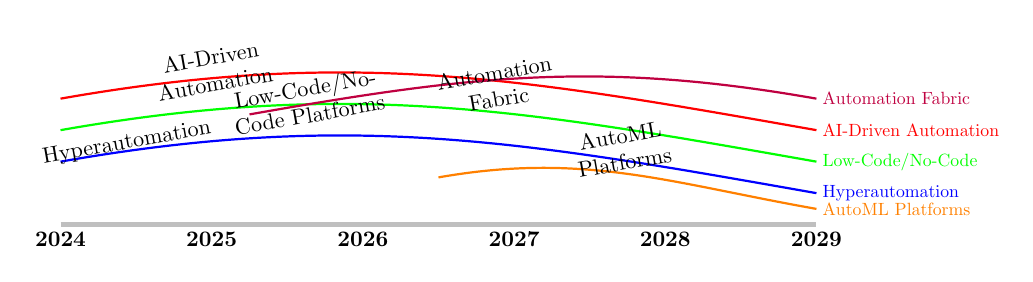
\begin{tikzpicture}[scale=0.8, transform shape]
        % Timeline
    \draw[-, ultra thick, draw=gray!50] (0,0) -- (12,0);

    % Years
    \foreach \x/\year in {0/2024, 2.4/2025, 4.8/2026, 7.2/2027, 9.6/2028, 12/2029}
    \node[below] at (\x,0) {\textbf{\year}};

    % Trend lines
    \draw[thick, blue] (0,1) to[out=10, in=170] (12,0.5);
    \draw[thick, red] (0,2) to[out=10, in=170] (12,1.5);
    \draw[thick, green] (0,1.5) to[out=10, in=170] (12,1);
    \draw[thick, purple] (3,1.75) to[out=10, in=170] (12,2);
    \draw[thick, orange] (6,0.75) to[out=10, in=170] (12,0.25);

    % Trend labels (rotated for better fit)
    \node[above, text width=2.5cm, align=center, rotate=10] at (1,1) {Hyperautomation};
    \node[above, text width=2.5cm, align=center, rotate=10] at (2.5,2) {AI-Driven Automation};
    \node[above, text width=2.5cm, align=center, rotate=10] at (4,1.5) {Low-Code/No-Code Platforms};
    \node[above, text width=2.5cm, align=center, rotate=10] at (7,1.75) {Automation Fabric};
    \node[above, text width=2.5cm, align=center, rotate=10] at (9,0.75) {AutoML Platforms};

    % Legend
    \node[right, blue, scale=0.8] at (12,0.5) {Hyperautomation};
    \node[right, red, scale=0.8] at (12,1.5) {AI-Driven Automation};
    \node[right, green, scale=0.8] at (12,1) {Low-Code/No-Code};
    \node[right, purple, scale=0.8] at (12,2) {Automation Fabric};
    \node[right, orange, scale=0.8] at (12,0.25) {AutoML Platforms};
\end{tikzpicture}


\section{Skills to Develop for the AI-Augmented Consultant}

To succeed in the future of IT consulting, you'll need to cultivate a balance of technical prowess and soft skills. This combination will allow you to not only implement cutting-edge solutions but also guide your clients through the complexities of digital transformation.

\subsection{Technical Skills}

Focus on developing expertise in:

\begin{itemize}
    \item AI and Machine Learning: Understanding of core concepts, ability to implement and manage AI-driven automations
    \item Data Analysis and Visualization: Proficiency in tools like Python, R, Tableau, or Power BI
    \item Cloud Computing: Expertise in major platforms (AWS, Azure, Google Cloud) and cloud-native technologies
    \item Cybersecurity: Knowledge of security best practices for automated systems and AI models
    \item Low-Code/No-Code Development: Proficiency in platforms like n8n, Bubble, or Microsoft Power Platform
\end{itemize}

\subsection{Soft Skills}

Cultivate these abilities:

\begin{itemize}
    \item Adaptability and Continuous Learning: Ability to quickly learn and apply new technologies
    \item Strategic Thinking: Skill in aligning automation initiatives with business goals
    \item Ethical Decision Making: Capability to navigate complex ethical considerations in AI and automation
    \item Communication and Storytelling: Ability to explain complex technical concepts to non-technical stakeholders
    \item Change Management: Expertise in guiding organizations through digital transformation
\end{itemize}

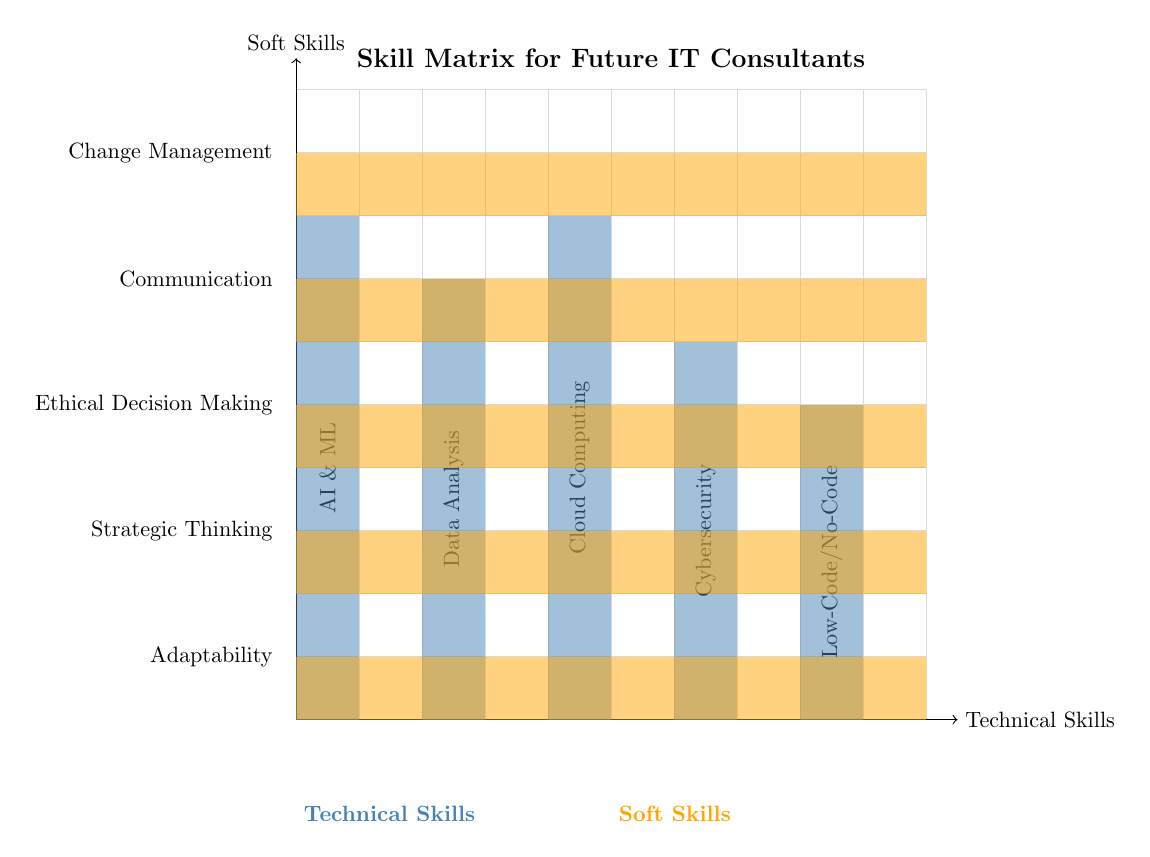
\begin{tikzpicture}[scale=0.8, transform shape]
        % Define colors
    \definecolor{techcolor}{RGB}{70,130,180} % Steel Blue
    \definecolor{softcolor}{RGB}{255,165,0} % Orange
    \definecolor{textcolor}{RGB}{0,0,0} % Black for text

    % Create the main grid
    \draw[step=1cm,gray!30,very thin] (0,0) grid (10,10);

    % Draw axes
    \draw[->] (0,0) -- (10.5,0) node[right] {Technical Skills};
    \draw[->] (0,0) -- (0,10.5) node[above] {Soft Skills};

    % Technical skills (centered on bars)
    \node[textcolor, rotate=90, anchor=center] at (0.5,4) {AI \& ML};
    \node[textcolor, rotate=90, anchor=center] at (2.5,3.5) {Data Analysis};
    \node[textcolor, rotate=90, anchor=center] at (4.5,4) {Cloud Computing};
    \node[textcolor, rotate=90, anchor=center] at (6.5,3) {Cybersecurity};
    \node[textcolor, rotate=90, anchor=center] at (8.5,2.5) {Low-Code/No-Code};

    % Soft skills
    \node[textcolor, anchor=east] at (-0.25,1) {Adaptability};
    \node[textcolor, anchor=east] at (-0.25,3) {Strategic Thinking};
    \node[textcolor, anchor=east] at (-0.25,5) {Ethical Decision Making};
    \node[textcolor, anchor=east] at (-0.25,7) {Communication};
    \node[textcolor, anchor=east] at (-0.25,9) {Change Management};

    % Skill levels
    \fill[techcolor,opacity=0.5] (0,0) rectangle (1,8);
    \fill[techcolor,opacity=0.5] (2,0) rectangle (3,7);
    \fill[techcolor,opacity=0.5] (4,0) rectangle (5,8);
    \fill[techcolor,opacity=0.5] (6,0) rectangle (7,6);
    \fill[techcolor,opacity=0.5] (8,0) rectangle (9,5);

    \fill[softcolor,opacity=0.5] (0,0) rectangle (10,1);
    \fill[softcolor,opacity=0.5] (0,2) rectangle (10,3);
    \fill[softcolor,opacity=0.5] (0,4) rectangle (10,5);
    \fill[softcolor,opacity=0.5] (0,6) rectangle (10,7);
    \fill[softcolor,opacity=0.5] (0,8) rectangle (10,9);

    % Title
    \node[font=\large\bfseries] at (5,10.5) {Skill Matrix for Future IT Consultants};

    % Legend
    \node[techcolor, anchor=west] at (0,-1.5) {\textbf{Technical Skills}};
    \node[softcolor, anchor=west] at (5,-1.5) {\textbf{Soft Skills}};
\end{tikzpicture}


\section{Ethical Considerations and Best Practices}

As automation and AI become more prevalent, ethical considerations become increasingly important. As an IT consultant, you'll need to guide your clients through these complex issues.

\subsection{Data Privacy and Security}

Key considerations include:

\begin{itemize}
    \item Implement privacy-by-design principles in all automation projects
    \item Stay updated on data protection regulations (GDPR, CCPA, etc.) and ensure compliance
    \item Regularly audit automated systems for potential security vulnerabilities
\end{itemize}

\subsection{Job Displacement and Workforce Transition}

Consider these strategies:

\begin{itemize}
    \item Develop strategies to reskill and upskill employees affected by automation
    \item Collaborate with HR to create new roles that complement automated systems
    \item Communicate transparently about the impact of automation on jobs
\end{itemize}

\subsection{Algorithmic Bias}

Key actions include:

\begin{itemize}
    \item Regularly test AI models for bias and fairness
    \item Ensure diverse representation in teams developing AI and automation solutions
    \item Implement explainable AI techniques to understand and mitigate bias
\end{itemize}

\begin{tikzpicture}
    [
    scale=0.7, transform shape,
    node distance = 1.5cm and 2cm,
    box/.style = {rectangle, draw, rounded corners, minimum width=2.5cm, minimum height=0.8cm, align=center, font=\small},
    decision/.style = {diamond, draw, aspect=2, minimum width=2.5cm, align=center, font=\small},
    arrow/.style = {->, >=stealth, thin}
    ]

% Start node
    \node[box] (start) {Start Automation Project};

% First decision
    \node[decision, below=of start] (privacy) {Involves\\ sensitive data?};

% Privacy branch
    \node[box, below left=of privacy] (data_protection) {Implement data\\ protection};
    \node[box, below=of data_protection] (privacy_audit) {Conduct privacy\\ assessment};

% Job impact decision
    \node[decision, below right=of privacy] (job_impact) {Impacts\\ existing jobs?};

% Job impact branch
    \node[box, right=of job_impact] (transition_plan) {Develop transition\\ plan};
    \node[box, below=of transition_plan] (communicate) {Communicate\\ changes};

% AI decision
    \node[decision, below=of job_impact] (ai_decision) {Uses AI/ML\\ models?};

% AI branch
    \node[box, below left=of ai_decision] (bias_check) {Check for\\ algorithmic bias};
    \node[box, below right=of ai_decision] (explainable) {Implement\\ explainable AI};

% Final steps
    \node[box, below=2cm of ai_decision] (review) {Review with\\ stakeholders};
    \node[box, below=of review] (implement) {Implement with\\ ethical safeguards};

% Arrows
    \draw[arrow] (start) -- (privacy);
    \draw[arrow] (privacy) -- node[left, font=\tiny] {Yes} (data_protection);
    \draw[arrow] (data_protection) -- (privacy_audit);
    \draw[arrow] (privacy) -- node[right, font=\tiny] {No} (job_impact);
    \draw[arrow] (job_impact) -- node[above, font=\tiny] {Yes} (transition_plan);
    \draw[arrow] (transition_plan) -- (communicate);
    \draw[arrow] (job_impact) -- node[right, font=\tiny] {No} (ai_decision);
    \draw[arrow] (ai_decision) -- node[left, font=\tiny] {Yes} (bias_check);
    \draw[arrow] (ai_decision) -- node[right, font=\tiny] {Yes} (explainable);
    \draw[arrow] (privacy_audit) |- (review);
    \draw[arrow] (communicate) |- (review);
    \draw[arrow] (bias_check) -- (review);
    \draw[arrow] (explainable) -- (review);
    \draw[arrow] (ai_decision) -- node[right, font=\tiny] {No} (review);
    \draw[arrow] (review) -- (implement);

\end{tikzpicture}


\section{Staying Adaptable and Continuously Learning}

In the fast-paced world of IT consulting, the ability to learn and adapt quickly is perhaps your most valuable asset. Here are strategies to stay current and continuously expand your knowledge base.

\subsection{Leveraging Online Learning Platforms}

\begin{itemize}
    \item Coursera, edX, and Udacity for structured courses in emerging technologies
    \item Pluralsight and LinkedIn Learning for hands-on technical skills
    \item YouTube channels and podcasts for staying updated on industry trends
\end{itemize}

\subsection{Engaging with Professional Communities}

\begin{itemize}
    \item Join relevant LinkedIn groups and participate in discussions
    \item Contribute to open-source projects on GitHub
    \item Attend virtual conferences and webinars in your areas of expertise
\end{itemize}

\subsection{Developing a Personal Learning System}

\begin{itemize}
    \item Use tools like Notion or Obsidian to create a personal knowledge base
    \item Implement spaced repetition techniques for retaining new information
    \item Set aside dedicated time each week for learning and experimentation
\end{itemize}

% TODO @screenshot: Example of a personal learning dashboard in Notion or a similar tool


\section{Potential Challenges and Adaptation Strategies}

As the IT consulting landscape evolves, several challenges may emerge. By anticipating these challenges, you can develop strategies to not only overcome them but to thrive in the face of change.

\subsection{Increased Competition from AI Tools}

\textbf{Challenge:} AI-powered tools may automate some traditional consulting tasks, potentially reducing the demand for certain services.

\textbf{Adaptation:}
\begin{itemize}
    \item Focus on high-value, strategic consulting that AI can't easily replicate
    \item Develop expertise in implementing and customizing AI tools for clients
    \item Position yourself as an "AI-human collaboration" expert, showcasing how human insight can enhance AI capabilities
\end{itemize}

\subsection{Changing Client Expectations}

\textbf{Challenge:} Clients may expect faster results and more personalized solutions, driven by the capabilities of AI and automation.

\textbf{Adaptation:}
\begin{itemize}
    \item Leverage automation tools to speed up your own workflows
    \item Develop a modular approach to consulting, allowing for rapid customization
    \item Invest in data analytics to provide more personalized insights
\end{itemize}

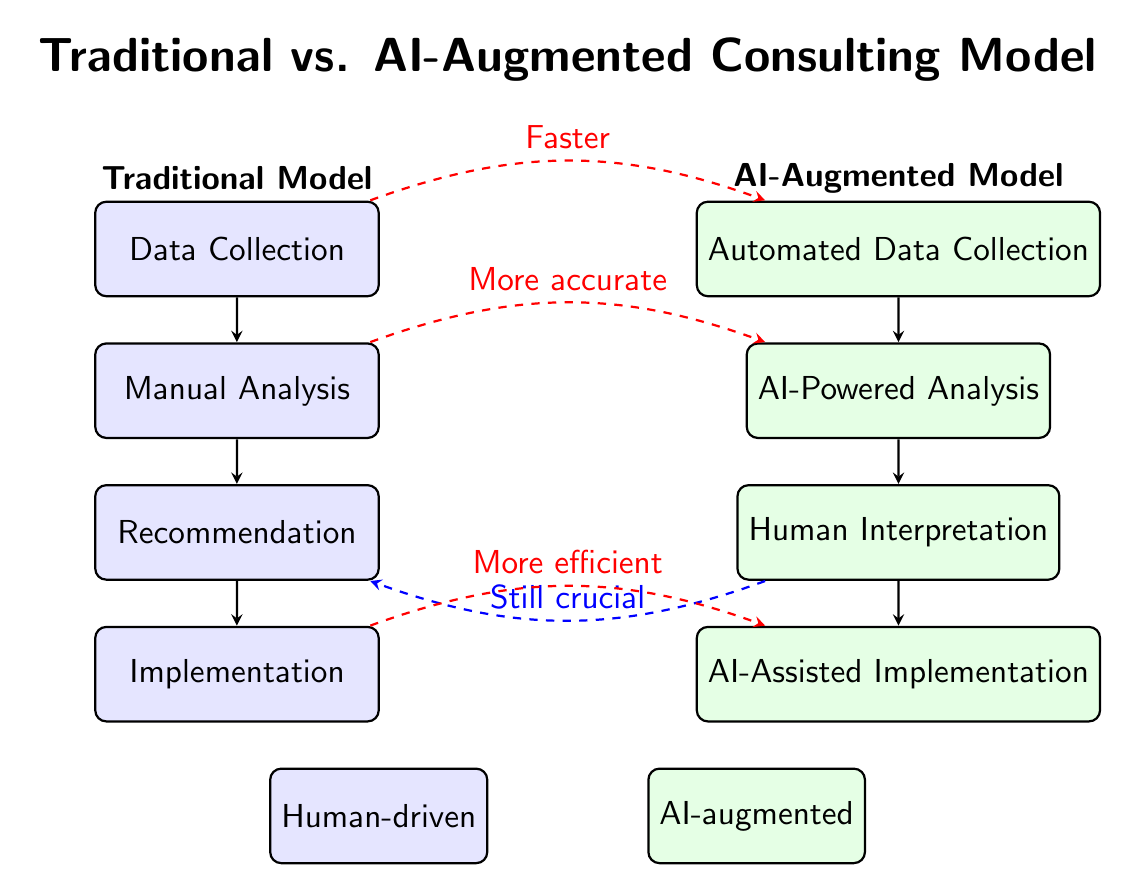
\begin{tikzpicture}
    [
    scale=1.2,
    transform shape,
    node distance=1.5cm and 4cm,
    box/.style={
        rectangle,
        rounded corners,
        draw=black,
        thick,
        minimum width=3cm,
        minimum height=1cm,
        text centered,
        font=\sffamily
    },
    trad/.style={box, fill=blue!10},
    ai/.style={box, fill=green!10},
    arrow/.style={->, >=stealth, thick},
    compare/.style={->, >=stealth, thick, dashed, bend left=20}
    ]

% Title
    \node[font=\sffamily\Large\bfseries] at (0,5) {Traditional vs. AI-Augmented Consulting Model};

% Traditional Model
    \node[font=\sffamily\bfseries] at (-3.5,3.75) {Traditional Model};
    \node[trad] (t1) at (-3.5,3) {Data Collection};
    \node[trad] (t2) at (-3.5,1.5) {Manual Analysis};
    \node[trad] (t3) at (-3.5,0) {Recommendation};
    \node[trad] (t4) at (-3.5,-1.5) {Implementation};

    \draw[arrow] (t1) -- (t2);
    \draw[arrow] (t2) -- (t3);
    \draw[arrow] (t3) -- (t4);

% AI-Augmented Model
    \node[font=\sffamily\bfseries] at (3.5,3.75) {AI-Augmented Model};
    \node[ai] (a1) at (3.5,3) {Automated Data Collection};
    \node[ai] (a2) at (3.5,1.5) {AI-Powered Analysis};
    \node[ai] (a3) at (3.5,0) {Human Interpretation};
    \node[ai] (a4) at (3.5,-1.5) {AI-Assisted Implementation};

    \draw[arrow] (a1) -- (a2);
    \draw[arrow] (a2) -- (a3);
    \draw[arrow] (a3) -- (a4);

% Comparison arrows
    \draw[compare, red] (t1) to node[midway, above, font=\sffamily] {Faster} (a1);
    \draw[compare, red] (t2) to node[midway, above, font=\sffamily] {More accurate} (a2);
    \draw[compare, blue] (a3) to node[midway, above, font=\sffamily] {Still crucial} (t3);
    \draw[compare, red] (t4) to node[midway, above, font=\sffamily] {More efficient} (a4);

% Legend
    \node[trad, minimum width=2cm] at (-2,-3) {Human-driven};
    \node[ai, minimum width=2cm] at (2,-3) {AI-augmented};

\end{tikzpicture}


\section{Key Technologies and Platforms for Future-Ready Consultants}

To stay ahead in the field of IT consulting, it's important to familiarize yourself with emerging technologies that have the potential to reshape industries. Here are some key technologies to watch:

\subsection{Quantum Computing}

While still in its early stages, quantum computing may begin to impact certain areas of automation and optimization by 2029.

\textbf{Potential applications:} Complex simulations, cryptography, optimization problems

\subsection{Edge Computing and 5G}

The combination of edge computing and 5G networks will enable new types of distributed automations and real-time processing.

\textbf{Potential applications:} IoT device management, real-time data processing, augmented reality systems

\subsection{Blockchain for Enterprise}

Blockchain technology is moving beyond cryptocurrency to solve enterprise-level problems.

\textbf{Potential applications:} Supply chain tracking, secure data sharing, smart contracts

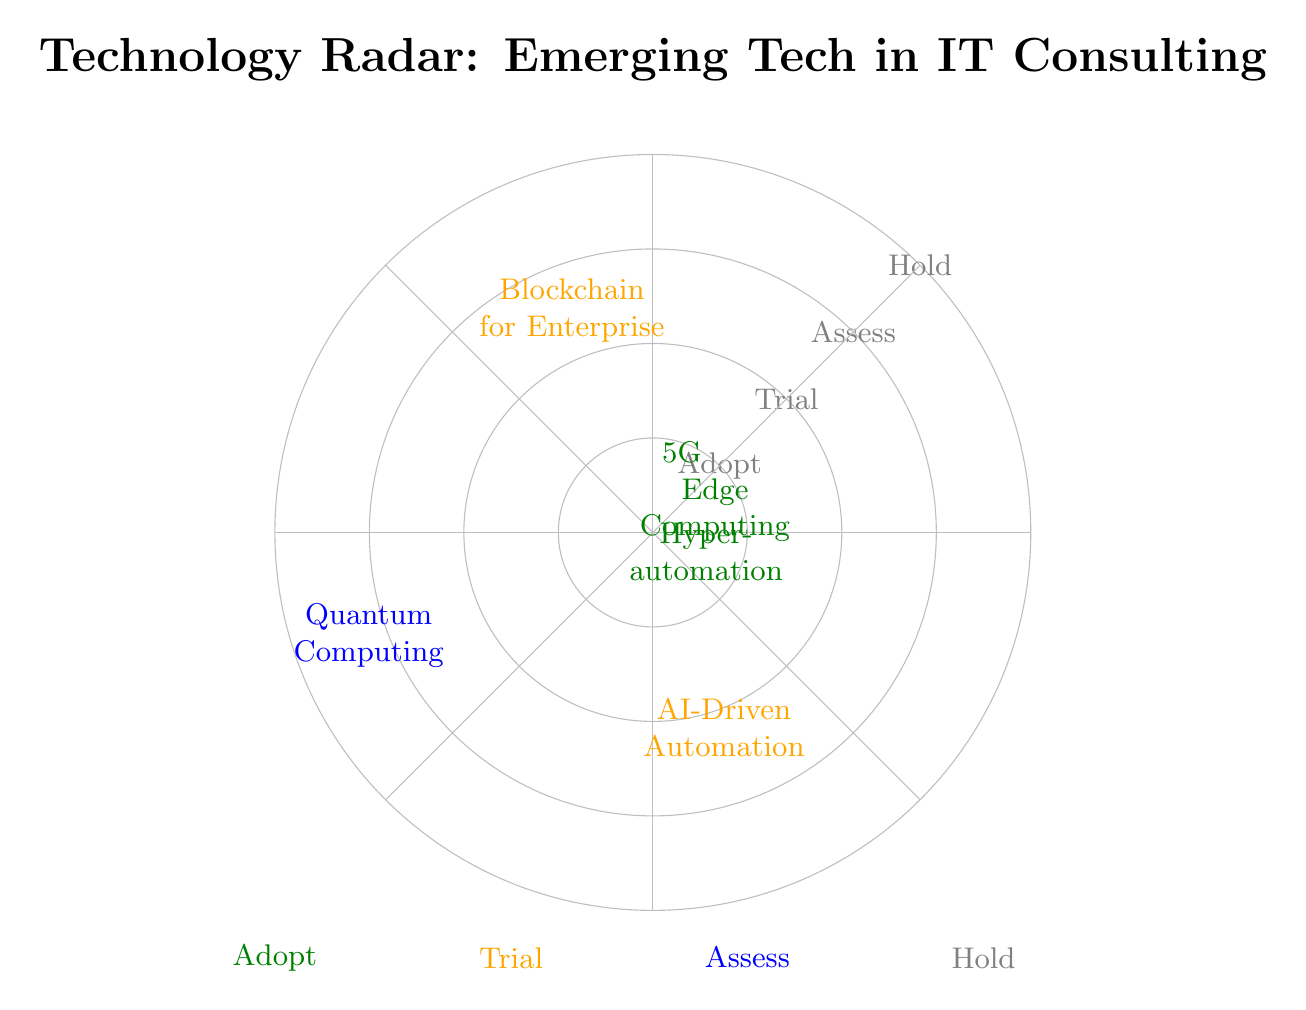
\begin{tikzpicture}[scale=1.2, transform shape]
        % Define colors
    \definecolor{adoptcolor}{RGB}{0,128,0}    % Green
    \definecolor{trialcolor}{RGB}{255,165,0}  % Orange
    \definecolor{assesscolor}{RGB}{0,0,255}   % Blue
    \definecolor{holdcolor}{RGB}{128,128,128} % Gray

    % Draw radar circles
    \foreach \r/\lbl in {4/Hold, 3/Assess, 2/Trial, 1/Adopt}
        {
        \draw[gray!50, thin] (0,0) circle (\r cm);
        \node[font=\small, gray] at (45:\r) {\lbl};
    }

    % Draw sector lines
    \foreach \angle in {0,45,...,315}
        {
        \draw[gray!50, thin] (0,0) -- (\angle:4);
    }

    % Plot technologies with adjusted positions and text wrapping
    \node[adoptcolor, font=\small, text width=2cm, align=center] at (20:0.7) {Edge Computing};
    \node[adoptcolor, font=\small, text width=1cm, align=center] at (70:0.9) {5G};
    \node[trialcolor, font=\small, text width=2.5cm, align=center] at (110:2.5) {Blockchain for Enterprise};
    \node[assesscolor, font=\small, text width=2.5cm, align=center] at (200:3.2) {Quantum Computing};
    \node[trialcolor, font=\small, text width=2.5cm, align=center] at (290:2.2) {AI-Driven Automation};
    \node[adoptcolor, font=\small, text width=2cm, align=center] at (340:0.6) {Hyper- automation};

    % Title
    \node[font=\Large\bfseries] at (0,5) {Technology Radar: Emerging Tech in IT Consulting};

    % Legend
    \node[adoptcolor, font=\small] at (-4,-4.5) {Adopt};
    \node[trialcolor, font=\small] at (-1.5,-4.5) {Trial};
    \node[assesscolor, font=\small] at (1,-4.5) {Assess};
    \node[holdcolor, font=\small] at (3.5,-4.5) {Hold};
\end{tikzpicture}


\section{Conclusion}

The future of IT consulting is bright for those who embrace change and continue to evolve. By staying informed about emerging trends, developing a balanced skill set, addressing ethical considerations, committing to continuous learning, and adapting to new challenges, you'll position yourself as an indispensable partner to your clients in the age of AI and automation.

Remember, the key to future-proofing your career is not just about mastering specific technologies, but about cultivating a mindset of curiosity, adaptability, and ethical responsibility. As you move forward, strive to be not just a consultant, but a visionary guide helping your clients navigate the exciting and sometimes uncertain waters of technological change.

\textbf{Action Items:}
\begin{enumerate}
    \item Conduct a self-assessment of your current skills and identify areas for improvement
    \item Choose one emerging technology from this chapter and create a 30-day learning plan
    \item Join at least two online communities related to your areas of expertise
    \item Start a "future trends" document to track developments in your industry
\end{enumerate}

% TODO @qr: QR code linking to additional resources on future trends in IT consulting and automation

By taking these steps and continuously refining your approach, you'll ensure that your IT consulting career remains vibrant, relevant, and impactful for years to come.